\iflanguage{ngerman}
{\chapter{Einleitung}}
{\chapter{Record of Work}}

\label{sec:outline}
This is a work record created before the actual thesis, which serves to scrutinize and list all possible contents that can be covered by the actual thesis. It contains work of the author that was conducted recently . As the professor's request, these work have to be properly recorded and preserved.

\section{Digit Sensor}
{\Large\color{red} Shall be moved to introduction part}

As Professor Aßmann suggested, the possibility of using \texttt{DIGIT} sensor \cite{Mike2020} to sense the attitude of pick components is the first matter that has to be figured out. Since the sensor was never experimented in the lab of Software Technology group until Professor Roberto Calandra become a faculty member at TU Dresden. We first have to conduct basic experiments to find out what it actually can do. To be specific, what features of various fabrics this sensor can capture and how we can interpret these captured features. Thus, we need to transform the raw data into fathomable variables that can be integrated into \texttt{ROS} systems. Eventually, combining the sensor with our robots that can serve to pick actual bricks for constructions.

\subsection{Test with Digit Sensor}
According to the definition given by \cite{Mike2020}, \texttt{DIGIT} is a "vision-based tactile sensor". It captures light reflection on elastic gel due to the deformation of elastomers that has physical contact with the object that we want to sense. It is supposedly good at identifying tactile because it doesn't use camera directly to discern features, but instead utilizing an intermediary material that can reflect tactile features.

\begin{figure}[t]
	\centering
	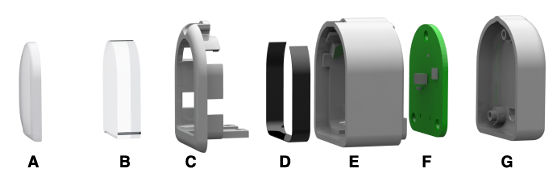
\includegraphics[width=1\textwidth]{fig/digit_components.png}
	\caption{Exploded view of a single DIGIT sensor. A) elastomer, B) acrylic window, C) snap-fit holder, D) lighting PCB, E) plastic housing, F) camera PCB, G) back housing.}
	\label{fig:digit} % Place the label after the caption
\end{figure}

Couple experiments have been conducted in the lab of Software Technology group. First, common fabrics such as cotton tee shirt and pine wood bricks are tested.

\begin{figure}[t]
	\centering
	\begin{subfigure}[t]{0.4\textwidth}
		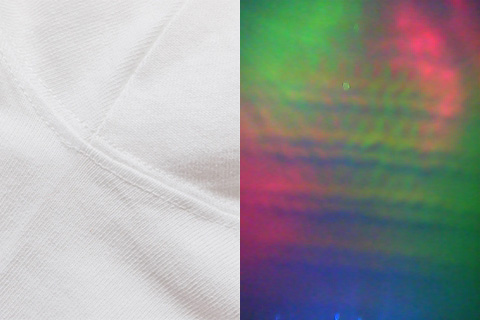
\includegraphics[width=1\textwidth]{fig/digit_cotton_shirt.jpg}
	\end{subfigure}
	\begin{subfigure}[t]{0.4\textwidth}
		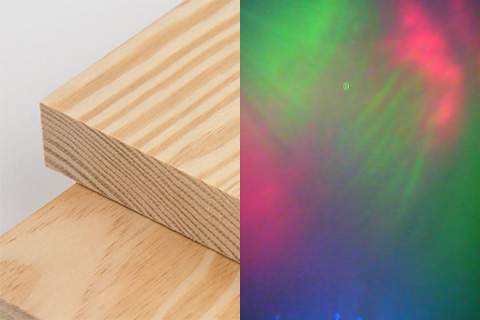
\includegraphics[width=1\textwidth]{fig/digit_pine_wood.jpg}
	\end{subfigure}
\caption{Object under test and corresponding raw measurements taken using DIGIT.}
\label{fig:texture}
\end{figure}

As figure \ref{fig:texture} illustrates, it clearly captures sub-millimeters textures that are normally indiscernible for cameras. Additionally, we tested the sensor performance under different ambient light conditions. \texttt{DIGIT} with LED self-illumination device ensures that the captured images are less affected by changes in ambient light, which means it can output stable features. 

\section{SHCC Frame Modules}
{\Large\color{red} Shall be moved to introduction part}

Next up, in our common use case, the \texttt{FRANKA} robot utilizes a gripper that has a pair of claws which can pick and drop objects by gripping. We want to test the scenario where grippers of a robotic hand are equipped with \texttt{DIGIT} sensors. In order to test the feasibility of mounting two sensor at the same time, we envisaged a scenario where interference might occur when the objects in contact with two sensors are too thin. This could potentially lead to mutual interference between the elastomers of two sensors, affecting imaging. After testing thin fabrics such as cotton and polyester. It can be confirmed that the interference between the two sensors can be neglected.

Having tested the basic performance of a digit sensor. We decided to further explore its capability by applying it to our current project, bridge frame modules. This is used to construct an arch structure to support subsequent bridge construction. We first assemble blocks that will be utilized for supporting frame modules. This part of construction is already implemented by {\LARGE\color{red} Wanqi Zhao's algorithms}. On top of the brick blocks, we will then build the bridge frame modules which is a simple version of \cite{IVANIUK2022}.

\begin{figure}[t]
	\centering
	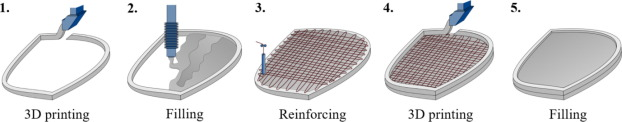
\includegraphics[width=1\textwidth]{fig/composites.jpg}
	\caption{Production Steps of Frame modules}
	\label{fig:composite} % Place the label after the caption
\end{figure}

\begin{figure}[t]
	\centering
	\begin{subfigure}[t]{0.4\textwidth}
		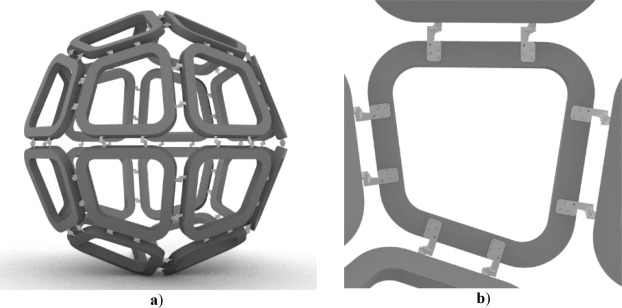
\includegraphics[width=1\textwidth]{fig/formwork.jpg}
	\end{subfigure}
	\begin{subfigure}[t]{0.4\textwidth}
		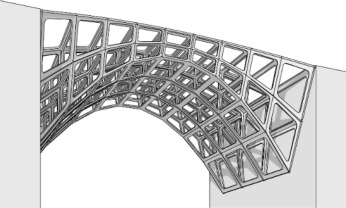
\includegraphics[width=1\textwidth]{fig/bridge.jpg}
	\end{subfigure}
	\caption{Space Frame Bridge built Using PQ-meshes}
	\label{fig:polyhedron}
\end{figure}

In figure \ref{fig:composite}, the production steps of frame module reveal that it has a composite structure. The peripheral part is made of metal and the interior is filled with "printable strain-hardening cement-based composites" \cite{IVANIUK2022}. These modules are normally created to have the shape of planar quadrilateral, because these PQ-meshes can approximate a great variety of freedom surfaces. Using identical PQ meshes, it is not difficult to build different polyhedron, which can contribute to building sophisticated constructions like a bridge as shown in figure \ref{fig:polyhedron}.

Theory aside, since we are not focusing on civil engineering or material science, the model we use in the laboratory is smaller in size compared to the one mentioned in the paper, and the connection method has been changed from the metal connector to magnetic connector.

\begin{figure}[t]
	\centering
	\begin{subfigure}[t]{0.45\textwidth}
		\centering
		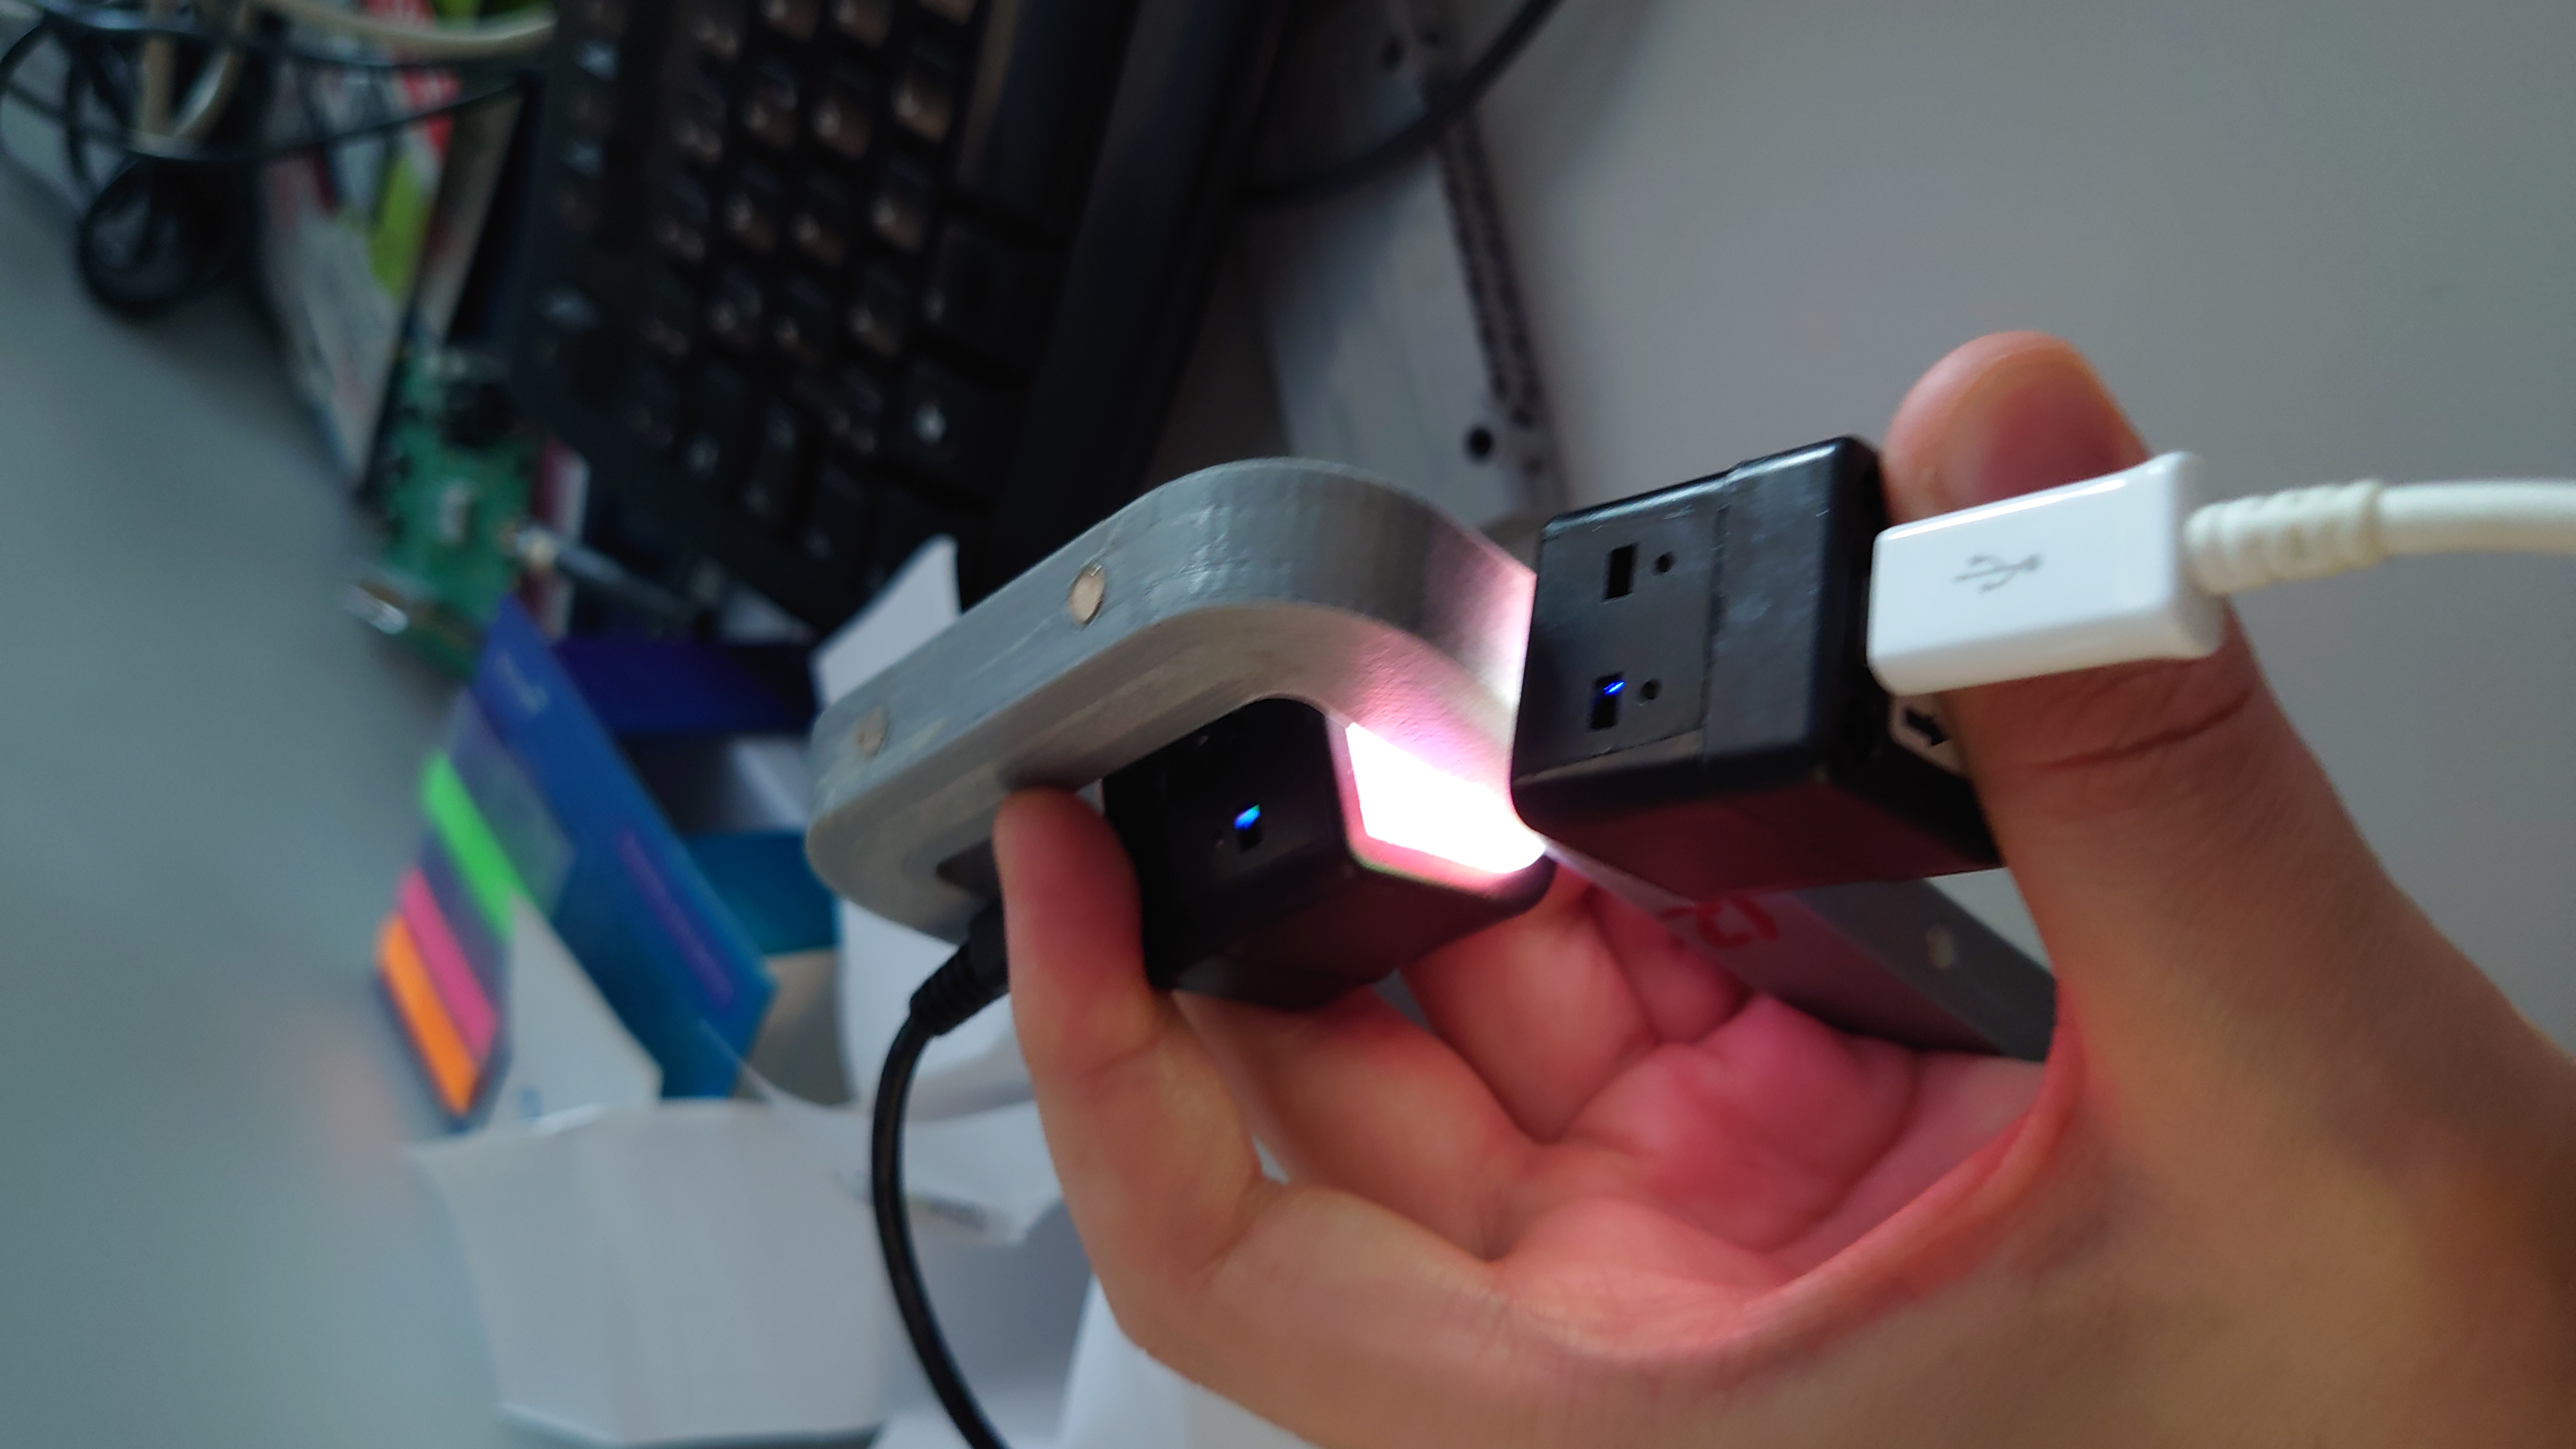
\includegraphics[height=3cm]{fig/vertical_overview.JPG} % Adjust height as needed
		\caption{Vertical grip overview}
	\end{subfigure}
	~ %add desired spacing between images, e. g. ~, \quad, \qquad, \hfill etc. 
	%(or a blank line to force the subfigure onto a new line)
	\begin{subfigure}[t]{0.45\textwidth}
		\centering
		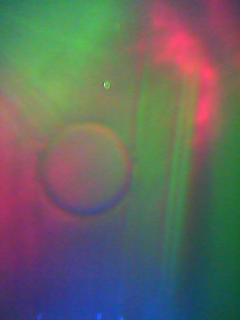
\includegraphics[height=3cm]{fig/vertical_digit.png} % Adjust height as needed
		\caption{Detail of the vertical grip with DIGIT sensor}
	\end{subfigure}
	\medskip % adds some vertical space between the rows of subfigures
	\begin{subfigure}[t]{0.45\textwidth}
		\centering
		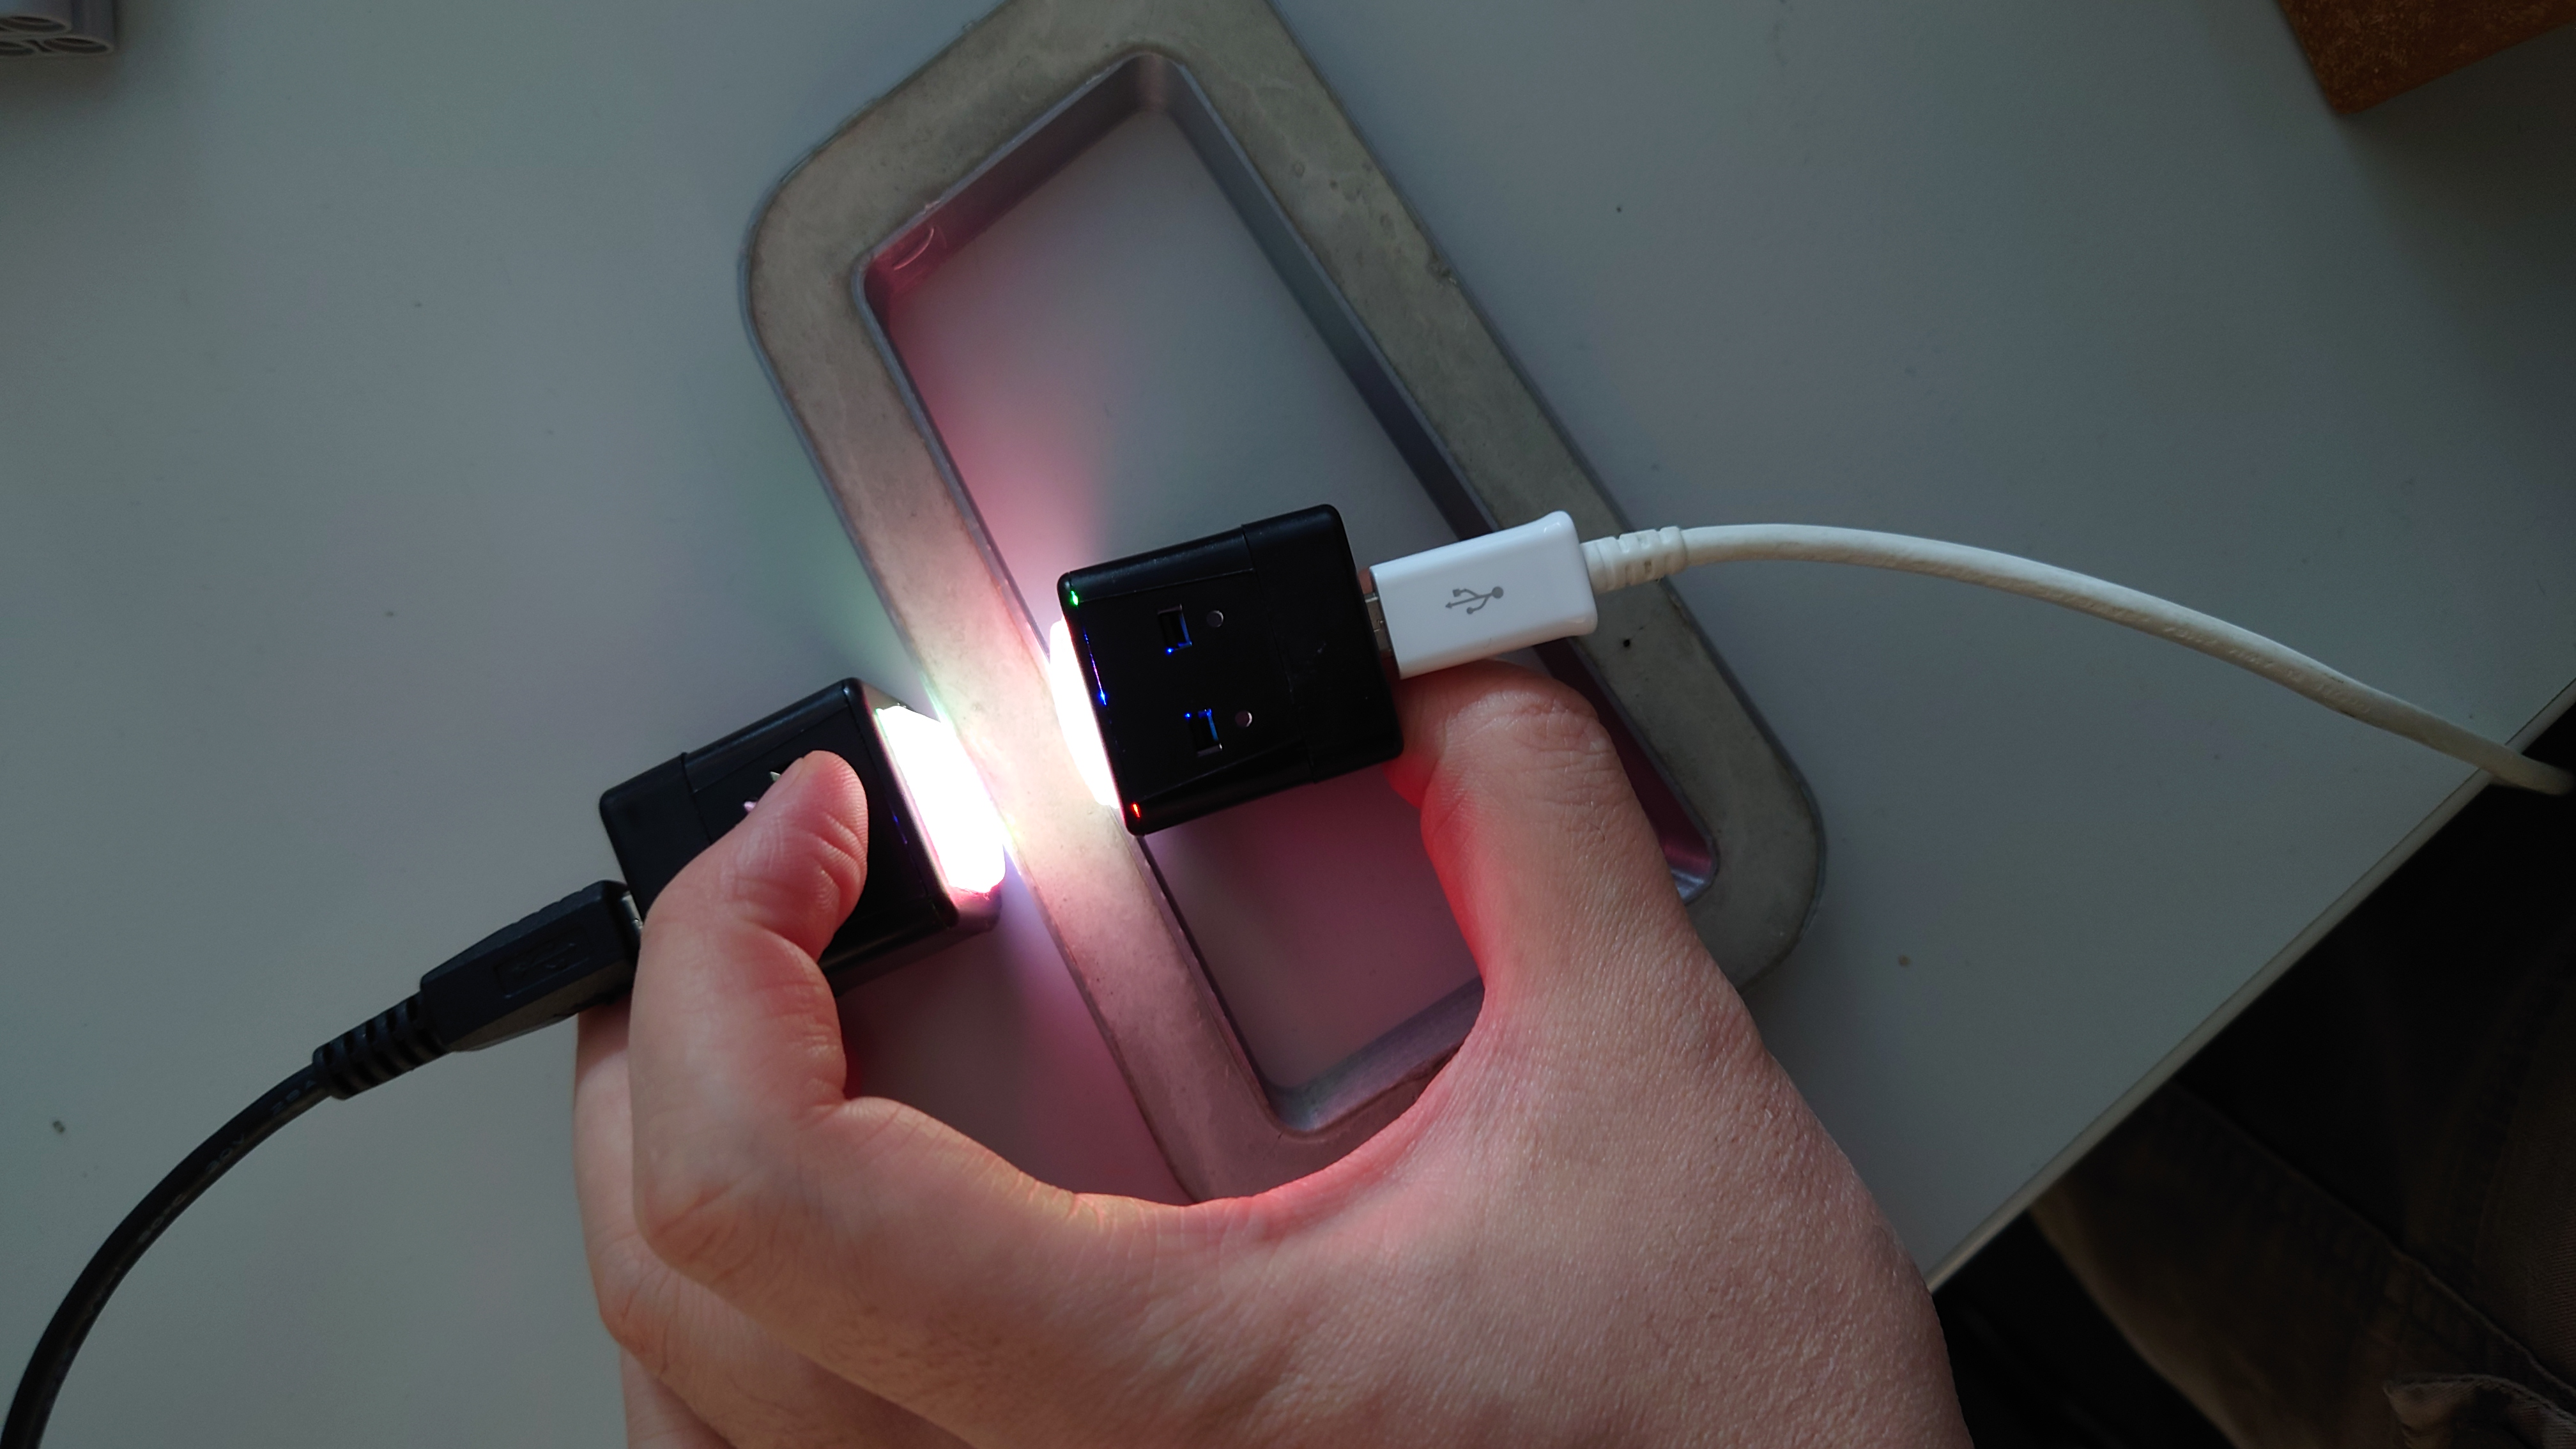
\includegraphics[height=3cm]{fig/perpendicular_overview.JPG} % Adjust height as needed
		\caption{Perpendicular grip overview}
	\end{subfigure}
	~ %add desired spacing between images, e. g. ~, \quad, \qquad, \hfill etc. 
	%(or a blank line to force the subfigure onto a new line)
	\begin{subfigure}[t]{0.45\textwidth}
		\centering
		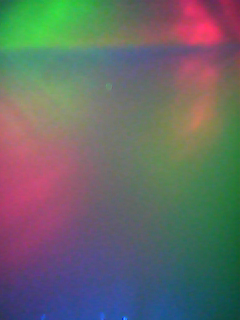
\includegraphics[height=3cm]{fig/perpendicular_digit.png} % Adjust height as needed
		\caption{Detail of the perpendicular grip with DIGIT sensor}
	\end{subfigure}
	\caption{Two Gripping Tests}
	\label{fig:griptest}
\end{figure}

\section{Image Processing}
\subsection{Test Design: First Approach}
In the first serie of experiments, two \texttt{DIGIT} sensors are squeezed with hands to clamp the module frame in between. A serie of experiments are conducted with different settings such as angles of sensors, surface of the frames, pressure etc. These experiments are conceived based on our understanding of the material and performance of the robot arm explained in former chapter. 

The irregular quadrilateral appearance of modules makes it difficult for the original Emika gripper to grasp, especially considering the DIGIT sensors that will be added later. Therefore, in order to testify the feasibility of grasping from different angles so that later when it is mounted on the actual gripper, we would have better understanding of the outcome image. So, in the testing phase, we assumed two scenarios to grasp objects from different angle, mainly vertical and perpendicular.

Also, a very important feature that I am looking for is the tactile pattern that is captured by the sensor. To find out how many are there and how many of them are distinguishable. It will be very important for the design of image processing algorithm that comes afterwards.

The only output source of a digit sensor is a real-time camera that observes the deformation of elastic gel that reflects LED light projection. Image processing methodologies are very important since they will be the solid base for the upcoming algorithms of edge, angle detection, auto grasp position adjust and eventually textile recognition.

\subsection{Test Design: Pre-process}
OpenCV (Open Computer Vision Library) on Python is a preferable and popular option for image processing. This library consists of around 2000+ optimized algorithms that are useful for computer vision and machine learning. 

As I have explained in the introduction part, \texttt{DIGIT} sensor contains a micro camera: Omnivision OVM7692, a 60 fps color CMOS hosting a microlens array with focal length 1.15 mm and depth of field
30 cm. As the size of cmos and lens being small, the quality of captured frames is going to be poor. Color noise can severely impact the results of image processing algorithms.
\begin{figure}[t]
	\centering
	\begin{subfigure}[t]{0.45\textwidth}
		\centering
		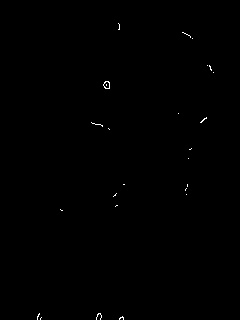
\includegraphics[height=3cm]{fig/vertical_edge.jpg} % Adjust height as needed
		\caption{Vertical grip edge detection result}
	\end{subfigure}
	~ %add desired spacing between images, e. g. ~, \quad, \qquad, \hfill etc. 
	%(or a blank line to force the subfigure onto a new line)
	\begin{subfigure}[t]{0.45\textwidth}
		\centering
		
\includegraphics[height=3cm]{fig/perpendicular_edge.jpg} % Adjust height as needed
		\caption{Perpendicular grip edge detection result}
	\end{subfigure}
	\caption{Two Edge Detection Results}
	\label{fig:edgedetection}
\end{figure}


